\section{Intermediate Representations}
\label{bg:sec:intermediate}

\Glspl{ir} are data structures designed to be independent of the machine
architecture and source language.  They are often invented with the intention
to ease program analysis and optimization in mind, by abstracting information
from the original program that are irrelevant to our objectives.  In this
section, we introduce several categories of existing \glspl{ir}, and delve
deeper into the advantages and disadvantages of each.

\subsection{Static Single Assignment Form and Control-Flow Graph}
\label{bg:sub:ssa_cfg}

Traditionally, \gls{ssa} form~\cite{alpern88, rau92} together with
the \gls{cfg} are used to represent data- and control-flow of a
program~\cite{cytron91}, because they are more favorable program
representations on which optimization passes can be implemented, when
compared to the original \gls{hll} or the output language.  \Gls{ssa} can be
advantageous in implementing conventional optimization techniques, \eg~code
motion~\cite{cytron86}, removing redundant computations~\cite{rosen88}, and
constant propagation~\cite{cytron91}.  Because the \gls{llvmir}~\cite{llvm_ir}
is based on \gls{ssa} and \glspl{cfg}, and is commonly used in many \gls{hls}
tools such as LegUp~\cite{legup}, we introduce \gls{ssa} and \glspl{cfg}
by compiling the dot-product example in Figure~\ref{bg:lst:dotprod} into
\gls{llvmir} as shown in Figure~\ref{bg:lst:dotprod_ll}.
\begin{figure}[ht]
    \centering
    \begin{lstlisting}[language=LLVM]
define float @dotprod(
    float* nocapture readonly %A,
    float* nocapture readonly %B) #0
{
; <label>:0
  br label %2

; <label>:1         ; preds = %2
  ret float %8

; <label>:2         ; preds = %2, %0
  %i.02 = phi i32 [ 0, %0 ], [ %9, %2 ]
  %d.01 = phi float [ 0.000000e+00, %0 ], [ %8, %2 ]
  %3 = getelementptr inbounds float, float* %A, i32 %i.02
  %4 = load float, float* %3, align 4, !tbaa !2
  %5 = getelementptr inbounds float, float* %B, i32 %i.02
  %6 = load float, float* %5, align 4, !tbaa !2
  %7 = fmul float %4, %6
  %8 = fadd float %d.01, %7
  %9 = add nuw nsw i32 %i.02, 1
  %exitcond = icmp eq i32 %9, 1024
  br i1 %exitcond, label %1, label %2
}
    \end{lstlisting}
    \caption{%
        The compiled and optimized \acrshort{llvmir} output from the
        dot-product example in Figure~\ref{bg:lst:dotprod}.
    }\label{bg:lst:dotprod_ll}
\end{figure}

The \gls{llvmir} of our example function consists of parts that are known
as \glspl{bb}.  Each \gls{bb} in turn often contains a label that uniquely
identifies the \gls{bb}, a list of \gls{llvmir} statements in \gls{ssa} form
without any branches, \ie~the statements are executed sequentially, and a
terminator instruction, which is typically a branch instruction that leads the
control-flow to a different \gls{bb}, by referencing a \gls{bb} label or a
function return.

The \gls{llvm} framework implicitly constructs a \gls{cfg} from the
\gls{ir} code, which is a directed graph representing the control-flow of
a program.  The vertices in the \gls{cfg} constitute \glspl{bb}, while
the edges indicate the control-flow directions (\ie~branches to other
\glspl{bb}), often with predicate attributes to determine whether the branch
is taken.  For instance, we consider the first line of the third \gls{bb} in
Figure~\ref{bg:lst:dotprod_ll}:
\begin{lstlisting}[language=LLVM]
    ; <label>:2     ; preds = %2 %0
\end{lstlisting}\vspace{-10pt}
which indicates it has a label value $2$ and the control-flow coming to this
\gls{bb} is from either \gls{bb}2 or \gls{bb}0, here we use \gls{bb}$n$ as a
shorthand denoting a \gls{bb} labelled $n$.  Additionally, this \gls{bb} ends
with the branch terminator instruction:
\begin{lstlisting}[language=LLVM]
    br i1 %exitcond, label %1, label %2
\end{lstlisting}\vspace{-10pt}
This instruction directs the control-flow to \gls{bb}1 or \gls{bb}2,
and the variable \verb|%exitcond| in the terminator instruction decides
which branch is taken.  Finally, the complete \gls{cfg} is shown in
Figure~\ref{bg:fig:dotprod_cfg}.  It is noteworthy that \gls{bb}2 has two edges
that leads to either \verb|BB1| or \verb|BB2| itself.  If \verb|%exitcond|
evaluates to false (\textbf{ff}), then another iteration of \gls{bb}2 will
commence, otherwise (\textbf{tt}) the exit condition is satisfied and will lead
the control-flow to \verb|BB1|.
\begin{figure}[ht]
    \centering
    \begin{tikzpicture}
        \node [] (entry) {\textbf{entry}};
        \node [rect, below of=entry, node distance=4em] (bb0) {\texttt{BB0}};
        \node [rect, below of=bb0, node distance=4em] (bb1) {\texttt{BB1}};
        \node [rect, below of=bb1, node distance=4em] (bb2) {\texttt{BB2}};
        \node [coordinate, right of=bb1, node distance=5em] (bb1tr) {};
        \node [coordinate, left of=bb2, node distance=8em] (bb2tl) {};
        \node [coordinate, right of=bb2, node distance=8em] (bb2tr) {};
        \node [below of=bb2, node distance=4em] (exit) {\textbf{exit}};
        \draw [->] (entry) -- (bb0);
        \draw [- ] (bb0)    to[out=0, in=90]    (bb1tr);
        \draw [->] (bb1tr)  to[out=-90, in=0]   (bb2);
        \draw [- ] (bb1)    to[out=180, in=90]  (bb2tl);
        \draw [->] (bb2tl)  to[out=-90, in=180] (exit);
        \draw [->] (bb2) -- node[auto, swap]{\textbf{tt}} (bb1);
        \draw [->] (bb2) to[out=-150, in=150, loop]
            node[auto, swap]{\textbf{ff}} (bb2);
    \end{tikzpicture}
    \caption{%
        The \acrshort{cfg} of the \acrshort{llvmir} code in
        Figure~\ref{bg:lst:dotprod_ll}.
    }\label{bg:fig:dotprod_cfg}
\end{figure}

Each \gls{bb} contains sequential computations that are represented by
\gls{ssa} instructions.  The \gls{ssa} form describes the operations in the
original program, such that each variable in it is assigned exactly one value.

The sequence of instructions that assigns to \verb|%3|-\verb|%9| in
Figure~\ref{bg:lst:dotprod_ll} carries out most of the computations in the
program.  It starts by reading \verb|A[i]| and \verb|B[i]|, multiplying them
together, then adding the result with \verb|d| to form a new variable, and
finally, the iteration value is incremented by $1$.  It may seem unusual that
the accumulated sum of products and the iteration value are not assigned
to \verb|d| and \verb|i| respectively.  We can imagine two \glspl{bb}, one
initializes \verb|d| and \verb|i| to zeros, the other accumulates these two
variables in a loop.  As all variables must be assigned once only, one of
the \glspl{bb} should use different names for these two variables.  When the
control-flows of these two \glspl{bb} join, we must introduce a way to read
from the variables that are assigned in the two \glspl{bb} in the succeeding
\gls{bb}\@.  A new instruction, called the $\phi$-function is therefore defined
for our purpose.  The $\phi$-function accepts two variable names as its inputs,
and produces the value of either variable as its output, determined by which
preceding \gls{bb} the control-flow came from.  For example, in \gls{llvmir},
the instruction:
\begin{lstlisting}[language=LLVM]
    %d.01 = phi float [ 0.000000e+00, %0 ], [ %8, %2 ]
\end{lstlisting}\vspace{-10pt}
shows that if the control-flow originated from \gls{bb}0, then a constant zero
is returned, otherwise the control-flow had to come from \gls{bb}2 and the
value of \verb|%8| is used instead.

The rationale of \gls{ssa} is that we can abstract away anti- and output
dependences by never assigning to the same variable twice, while only true
data-flow dependences remain.  An anti-dependence is a dependence relation
when a read operation must precede a write to the same variable, and an output
dependence is when two writes refer to the same location.  By removing these
dependences and deferring the analysis of them, certain program optimization
analyses can run much more efficiently.  Analyses that may benefit from this
include scheduling~\cite{rau94}, liveness analysis (estimating the lifetime
of variables to reduce register requirements)~\cite{cytron91}, detecting
opportunities for parallelism~\cite{cytron87}, and finding equivalent parts in
the program~\cite{alpern88}.

In a cyclic \gls{cfg}, the control-flow could potentially revisit a \gls{bb},
and instructions in this \gls{bb} will inevitably assign a different value to
the same variable, which forms anti- and output dependences, which could have
a detrimental effect on efficient loop pipelining in some computing machines.
An alternative \gls{ir}, the \gls{dsa} form~\cite{rau92} can therefore be used
in place of the \gls{ssa} to address this issue.  The \gls{dsa} defines a
linear sequence of virtual registers for each variable, such that every time
the variable is assigned in a dynamic execution path, a new virtual register is
used.

\subsubsection{Alternatives to \gls{ssa} and \gls{cfg}}

There are a number of alternative \glspl{ir} that are similar in construction
to the \gls{ssa} and \gls{cfg} approach in \gls{llvmir}\@.  For instance, the
data-dependence graph~\cite{rau94} introduced in Section~\ref{bg:sub:sdc} are
designed for the purpose of capturing data-flow dependences in polyhedral
methods. \gls{dfg} is a popular alternative to \gls{ssa}, which is often
a \gls{dag}.  In general, a \gls{dfg}'s vertices are input, output and
operation nodes, and the edges capture the dependences between these nodes.
A \glspl{dfg} however generally does not preserve enough information for us
to reconstruct a program from the graph itself.  A group of data structures,
known as \gls{cdfg}~\cite{orailoglu86}, is commonly used to represent programs
in \gls{hls} tools, \eg~SPARK~\cite{gupta04}.  A \gls{cdfg} resembles a
\gls{cfg} such as the one used in \gls{llvmir}, but in lieu of using sequential
instructions in \gls{ssa} form in graph vertices, each vertex contains a
\gls{dfg}, where no \gls{ssa} temporary variables are used and data-flow
dependences can by explicitly identified by edges.


\subsection{Equality Saturation}
\label{bg:sub:equality_saturation}

The \glspl{ir} we discussed above are all used to analyze and transform the
underlying program structure, so as to produce a new representation of the
optimized program.  In a conventional optimizing compiler, program optimization
is often carried out in a sequence of transformation passes, where each pass
accepts a program, often written in a certain \gls{ir}, and produces an
optimized program in the \gls{ir}\@.  The traditional practice is to always
apply these optimization phases in a fixed order, but a good ordering of these
phases is crucial to achieve a good optimized result, and the optimal ordering
varies across applications being compiled~\cite{almagor04}.  The process of
finding the optimal ordering is known as the \emph{phase-ordering problem},
which is in general undecidable~\cite{touati06}.  Moreover, programs running
on \glspl{cpu} or \glspl{gpu} are usually quantified by their throughput or
latency, in contrast, designs on \glspl{fpga} concern us with additional
objectives besides run time, such as power consumption and resource utilization
that impact the quality of synthesized circuit.  Multiple designs which
trade-off these objectives could exist, and which design to choose relies
on the specifics of the use case.  It is therefore sensible to explore the
design space by optimizing multiple objectives simultaneously.  For the above
reasons, it is desirable to have an \gls{ir} and the associated optimization
procedures to efficiently discover equivalent structures that lead to different
implementations of the original program.

In software, a novel approach called \emph{equality saturation} is proposed
in~\cite{tate09} to find multiple possible optimized variants of the original
program, and subsequently deal with the phase-ordering problem.  It creates a
new graph-based \gls{ir}, \gls{peg}, to encode the effects of executing the
program.

To begin, we review the structure of the \gls{peg}, by considering a simple
loop example in Figure~\ref{bg:fig:factorial}.  By understanding how the
\gls{peg} can be evaluated for the output values, we can interpret how the
\gls{peg} captures the control- and data-flow information of the program.
\glspl{peg}, similar to arithmetic expressions expressed in a tree structure,
can be evaluated in a bottom-up fashion, by recursively propagating computed
values from the leaf nodes to the root of the tree.  However, unlike arithmetic
expressions which are acyclic, edges in \glspl{peg} may form cycles to express
loops in the original program.
\begin{figure}[ht]
    \newsavebox{\factlstbox}
    \begin{lrbox}{\factlstbox}
    \begin{lstlisting}
int x = 1;
int y = 1;
while (y <= 10) {
    x = y * x;
    y = y + 1;
}
    \end{lstlisting}
    \end{lrbox}
    \centering
    \subfloat[The original program.]{%
        \begin{minipage}{0.4\textwidth}
            \usebox{\factlstbox}
        \end{minipage}\label{bg:lst:factorial_c}
    }
    \subfloat[The resulting \gls{peg}.]{%
        \begin{minipage}{0.5\textwidth}
        \begin{tikzpicture}[mir]
            \foreach \i/\v/\op in { 1/x/*, 2/y/+ } {
                \node (\v) [mirnode] at (\i * 30mm, 0) {$\v$};
                \node (e\i) [mirnode, right=of \v] {$\mathit{eval}_1$};
                \node (t\i) [mirnodealt, below left=of e\i, yshift=-10mm]
                    {$\theta_1$};
                \node (1\i) [mirnode, below left=of t\i] {$1$};
                \node (o\i) [mirnode, below right=of t\i] {\texttt{\op}};
                \draw[|->] (\v) -- (e\i);
                \draw[-] (e\i) -- (t\i.100);
                \draw[-] (t\i) -- (1\i);
                \node (mid\i) [coordinate, right=of o\i, yshift=-2mm] {};
                \draw[-] (t\i) -- (o\i)
                    to[out=-45, in=-135] (mid\i)
                    to[out=45, in=45] (t\i.60);
            }
            \node (12) [mirnode, below left=of o2] {$1$};
            \draw[-] (o2) -- (12);

            \node (p) [mirnode, below right=10mm of e2] {$\mathit{pass}_1$};
            \node (neg) [mirnode, below=of p] {$\neg$};
            \node (leq) [mirnode, below=of neg] {$\leq$};
            \node (10) [mirnode, below right=of leq] {$10$};
            \draw[-] (e1) to[out=-45, in=160] (p);
            \draw[-] (e2) -- (p.90);
            \draw[-] (p) -- (neg) -- (leq) -- (10);
            \node (mid3) [coordinate, left=12mm of neg] {};
            \draw[-] (leq) to[out=-135, in=-45] (mid3)
                           to[out=135, in=50] (t2.80);

            \node (mid4) [coordinate, below=5mm of o1, xshift=2mm] {};
            \draw[-] (o1) to[out=-135, in=180] (mid4) to[out=0, in=135] (t2);
        \end{tikzpicture}
        \end{minipage}\label{bg:fig:factorial_peg}
    }
    \caption{%
        A simple loop which computes the factorial of 10, and the resulting
        \acrshort{peg}\@.  This example and its \acrshort{peg}, showing
        computations that lead to the final \texttt{x} and \texttt{y}, is taken
        from~\cite{tate09}.
    }\label{bg:fig:factorial}
\end{figure}

\subsubsection{Data-Flow Nodes}

All loops in the \gls{peg} are formed by $\theta$ nodes, which is used in the
following form:
\begin{center}
    \vspace{-16.5pt}
    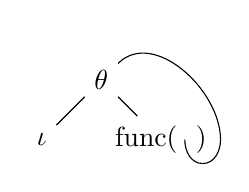
\begin{tikzpicture}
        \node (theta) at (0, 0) {$\theta$};
        \node (init) at (-5ex, -5ex) {$\iota$};
        \node (func) at (5ex, -5ex) {$\mathrm{func}(~~)$};
        \node[coordinate] (input) at (7ex, -5ex) {};
        \node[coordinate] (mid1) at (8.5ex, -7ex) {};
        \node[coordinate] (mid2) at (10ex, -5ex) {};
        \draw[-] (theta) -- (init);
        \draw[-] (theta) -- (func);
        \draw[-] (input) to[out=-90, in=180] (mid1);
        \draw[-] (mid1) to[out=0, in=-90] (mid2);
        \draw[-] (mid2) to[out=90, in=45] (theta);
    \end{tikzpicture}
    \vspace{-16.5pt}
\end{center}
where it accepts two child graphs, $\iota$ and $\mathrm{func}$, and
$\mathrm{func}$ further takes the $\theta$ node as one of its inputs to
form a complete cycle.  Evaluating a $\theta$ node produces a list of
values computed iteratively by the node's subgraph.  The first value in the
list, is the computed result of $\iota$, which we name $i$, and values in
the rest of the sequence are iteratively computed by $\mathrm{func}$.  In
functional programming, this is similar to iteratively computing the fixpoint
$\mathbf{fix}\,F$ of an initial list $[i]$, which is defined as:
\begin{equation}
    \mathbf{fix}\,F ([i]) = \lim_{n \to \infty} F^n ([i]),
    \quad\text{where~}
    F(v) = \mathrm{prepend}\left(
        i, \mathrm{map}\left( \mathrm{func}, v \right)
    \right).
\end{equation}
Here, $\mathrm{map}(\mathrm{func}, v)$ applies the subgraph computation
$\mathrm{func}$ to all elements in the list $v$, and $\mathrm{prepend}(i,
v^\prime)$ prepends the element $i$ to the list $v^\prime$.

For example, the following subgraph extracted from
Figure~\ref{bg:fig:factorial_peg} evaluates to the sequence $[1, 2, 3, 4,
\mathellipsis]$:
\begin{center}
    \vspace{-16.5pt}
    \begin{tikzpicture}
        \node (theta) at (0, 0) {$\theta_1$};
        \node (init) at (-5ex, -5ex) {$1$};
        \node (add) at (5ex, -5ex) {$+$};
        \node (one) at (0, -10ex) {$1$};
        \node[coordinate] (mid) at (8ex, -5ex) {};
        \draw[-] (theta) -- (init);
        \draw[-] (theta) -- (add);
        \draw[-] (add) -- (one);
        \draw[-] (add) to[out=-45, in=-90] (mid);
        \draw[-] (mid) to[out=90, in=45] (theta);
    \end{tikzpicture}
    \vspace{-16.5pt}
\end{center}

It is noteworthy that $\theta$ nodes may have subscripts.  For instance,
in Figure~\ref{bg:fig:factorial_peg}, both nodes $\theta_1$ share the same
subscript $1$.  This is used to indicate that the two sequences produced
by both $\theta$ nodes iterate simultaneously, \ie~they share the same
iteration count so that a new value for \verb|x| can be computed as we update
\verb|y|.  Therefore, the $\theta_1$ node in the left of this figure produces
a sequence of the factorials of $[1, 2, 3, \mathellipsis]$, \ie~$[1, 2, 6, 24,
\mathellipsis]$.

Computation nodes, such as arithmetic $+$ and Boolean operators $\leq$ and
$\neg$ in Figure~\ref{bg:fig:factorial_peg}, operates on a list of values, by
performing the computation on each value in the list.

For instance, the $\leq$ node accepts two inputs, the sequence $[1, 2, 3,
\mathellipsis]$ derived earlier, and a scalar $10$, computes the result of $x
\leq 10$ for each element $x$ in the sequence, and finally produces the list,
where $\truelit$ and $\falselit$ respectively denote true and false Boolean
values:
\begin{equation}
    [
        \truelit, \truelit, \truelit, \truelit, \truelit,
        \truelit, \truelit, \truelit, \truelit, \truelit,
        \falselit, \falselit, \falselit, \mathellipsis
    ].
\end{equation}
The subsequent $\neg$ node then negates all elements in the list:
\begin{equation}
    [
        \falselit, \falselit, \falselit, \falselit, \falselit,
        \falselit, \falselit, \falselit, \falselit, \falselit,
        \truelit, \truelit, \truelit, \mathellipsis
    ].
    \label{bg:eq:bool_seq}
\end{equation}

\subsubsection{Control-Flow Nodes}

The $\theta$ node encodes an infinite sequence of computed values, whereas
the output value of the program is a scalar.  By further representing
control-flow information in \gls{peg}, it becomes possible to refer to a
single value in this sequence, as the output of the program.  To do so,
Tate~\etal~\cite{tate09} further introduce $\mathrm{pass}$ and $\mathrm{eval}$
nodes.  The $\mathrm{pass}$ node finds the first true ($\truelit$) value
in a sequence of Boolean values, and returns the index of this value, and
$\mathrm{eval}$ takes two child nodes, where the first node evaluates to a list
$v$ of values, and the second is an scalar $n$ used to select a scalar value
from $l$, as the output of this node.

To illustrate, the $\mathrm{pass}_1$ node finds the first $\truelit$ in the
list~\eqref{bg:eq:bool_seq}, $11$.  The $\mathrm{eval}$ node of the output
variable \verb|y| subsequently fetches the $11$-th item from the list $[1, 2,
3, 4, \mathellipsis]$ we produced earlier, which is $11$.  Similarly we can
apply the same process to find that the output \verb|x| is \mbox{$10\,!\,$},
\ie~the factorial of $10$.

By using $\mathrm{pass}$ and $\mathrm{eval}$ nodes to represent the
control-flow in an algebraic fashion, and mixing data- and control-flows
together in the graphical representation, \glspl{peg} provide us with
greater opportunities to optimize data-flow across control-flow boundaries
and \emph{vice versa}.  Simple equivalence rules can be defined for these
nodes algebraically.  For instance, arithmetic operators can be distributed
over $\theta$ and $\mathrm{eval}$, \eg~$\mathrm{eval}(j, k) + i \equiv
\mathrm{eval}(j + i, k)$.  Complex transformations can therefore be deductively
constructed from these simple equivalence rules.

\subsubsection{Equivalence Finding}

By applying transformation passes to the \gls{peg}, their approach detects
incremental modifications, and appends these changes to the original
\gls{peg}\@.  The new changes, represented as extra structures in the
\gls{peg}, are linked to their corresponding equivalent nodes by equivalence
edges.  These edges indicate a pair of subgraphs are equivalent, forming a
\gls{epeg}, that could capture multiple \glspl{peg} in the same structure.  The
resulting \gls{epeg} is similar to the one in Figure~\ref{bg:fig:epeg}, where
dashed edges indicate equivalences.  It is notable that each edge allows a
binary choice, therefore the number of \glspl{peg} can be represented in an
\gls{epeg} could be exponential in the number of equivalence edges.
\begin{figure}[ht]
    \centering
    \begin{tikzpicture}[mir]
        \node (*1) [mirnode] at (0, 0) {$*$};
        \node (t1) [mirnodealt, below left=10mm of *1] {$\theta$};
        \node (51) [mirnode, below right=of *1] {$5$};
        \node (01) [mirnode, below left=of t1] {$0$};
        \node (f1) [mirnode, below right=of t1] {$\phi$};
        \node (d1) [mirnode, below left=of f1] {$\delta$};
        \node (+1) [mirnodealt, below=5mm of f1] {$+$};
        \node (31) [mirnode, below left=of +1] {$3$};
        \node (+2) [mirnodealt, below right=of +1] {$+$};
        \node (11) [mirnode, below left=of +2] {$1$};
        \draw[-] (*1) -- (t1.60);
        \draw[-] (*1) -- (51);
        \draw[-] (t1) -- (f1) -- (+1) -- (+2) -- (11);
        \draw[-] (t1) -- (01);
        \draw[-] (f1) -- (d1);
        \draw[-] (f1) to[bend left] (+2);
        \draw[-] (+1) -- (31);
        \draw[-] (+2) -- (11);
        \draw[-] (+2) to[out=-45, in=45, looseness=2] (t1);

        \node (t2) [mirnode, right=20mm of *1] {$\theta$};
        \draw[dashed] (*1) -- (t2);
        \node (*2) [mirnode, below left=of t2] {$*$};
        \node (02) [mirnode, right=of *2] {$0$};
        \node (03) [mirnode, below left=of *2] {$0$};
        \node (52) [mirnode, below right=of *2] {$5$};
        \draw[-] (t2) -- (*2) -- (03);
        \draw[-] (*2) -- (52);
        \draw[dashed] (*2) -- (02);

        \node (*3) [mirnode, below right=of t2] {$*$};
        \node (53) [mirnode, below right=of *3] {$5$};
        \draw[-] (t2) -- (*3) -- (53);
        \draw[-] (*3)
            .. controls ($(*3) +(-0.5,-1.5)$) and ($(f1) +(1,1)$) .. (f1);

        \node (f2) [mirnode, right=15mm of *3] {$\phi$};
        \node (d2) [mirnode, below left=of f2] {$\delta$};
        \node (*4) [mirnode, below=of f2] {$*$};
        \node (54) [mirnode, below right=of *4] {$5$};
        \draw[dashed] (*3) -- (f2);
        \draw[-] (f2) -- (*4) -- (54);
        \draw[-] (f2) -- (d2);
        \draw[-] (*4)
            .. controls ($(*4) +(-1,-1)$) and ($(+1) +(1,1)$) .. (+1);

        \node (+3) [mirnode, right=15mm of *4] {$+$};
        \node (*5) [mirnode, below left=of +3] {$*$};
        \node (*6) [mirnode, below right=of +3] {$*$};
        \node (151) [mirnode, right=of *5] {$15$};
        \node (32) [mirnode, below left=of *5] {$3$};
        \node (55) [mirnode, below right=of *5] {$5$};
        \node (56) [mirnode, below right=of *6] {$5$};
        \draw[dashed] (*4) -- (+3);
        \draw[dashed] (*5) -- (151);
        \draw[-] (+3) -- (*5) -- (32);
        \draw[-] (*5) -- (55);
        \draw[-] (f2)
            .. controls ($(f2) +(0.5,-0.5)$) and ($(*6) +(-.5,1.5)$) .. (*6)
            .. controls ($(*6) +(-1,-2)$) and ($(+2) +(1,1)$) .. (+2);
        \draw[-] (+3) -- (*6) -- (56);

        \node (+4) [mirnode, right=15mm of *6] {$+$};
        \node (*7) [mirnode, below left=of +4] {$*$};
        \node (57) [mirnode, right=of *7] {$5$};
        \node (12) [mirnode, below left=of *7] {$1$};
        \node (58) [mirnode, below right=of *7] {$5$};
        \draw[dashed] (*6) -- (+4);
        \node (m1) [coordinate, right=of +4] {};
        \draw[-] (+4) to[out=-45, in=-90, looseness=1.5] (m1)
            .. controls ($(m1) +(0,1)$) and ($ (t2) +(1,1)$) .. (t2);
        \draw[-] (+4) -- (*7) -- (12);
        \draw[-] (*7) -- (58);
        \draw[dashed] (*7) -- (57);
    \end{tikzpicture}
    \caption{%
        An simple \acrshort{epeg} example, taken from~\cite{tate09}.
    }\label{bg:fig:epeg}
\end{figure}

By repeatedly applying all possible passes to the \gls{epeg}, this graph will
eventually saturate, \ie~no more equivalent structure can be added to the graph
because all possible equivalences are now discovered.  This process and the
resulting \gls{epeg} is more space-time efficient than enumerating all possible
\glspl{peg} along the path, because \gls{epeg} encourages sharing common
subgraphs, even across equivalent edges.  This saturated graph can always be
produced regardless of in what order we apply the passes, hence preventing
the phase-ordering problem.  Furthermore, \gls{epeg} defers the decision
of whether an optimization should be committed until we have reached full
saturation, allowing the global optima to be discovered.  In contrast, because
each optimization pass in a conventional compiler is performed once, the
compilers must make the decision to commit changes immediately after applying
the optimization, which consequently often results in local optima.
